\chapter{Gesamtentwurf}

\section{Model}

\subsection{Private Klassen}
\begin{figure}[H]
\noindent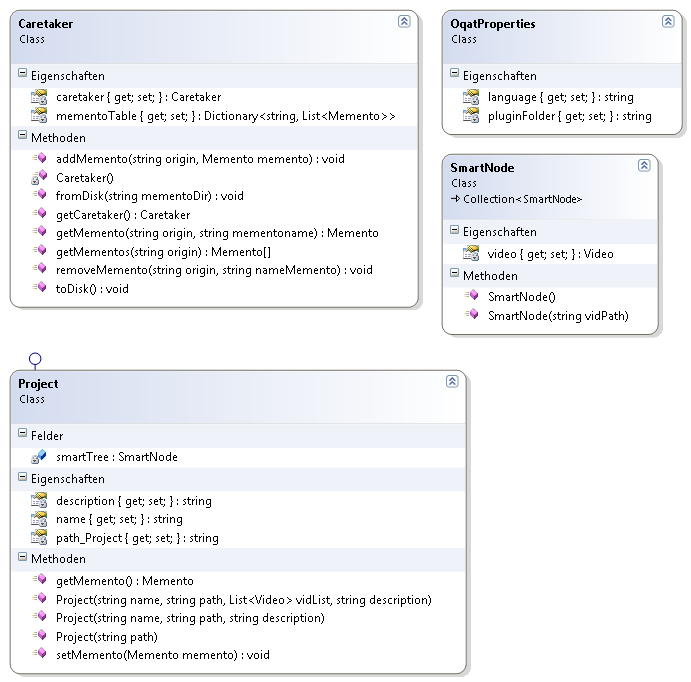
\includegraphics[scale=1]{bilder/Klassendiagramm/Model.png}
\label{Private Model A}
\caption{Model A}
\end{figure}

\class{Project}{Klasse}
Alle für das Projekt relevanten Daten befinden sich hier. Dies beinhaltet einen Pfad, einen Namen und eine Beschreibung. IMemorizable wird implementiert.


\class{OqatProperties}{Klasse}
Dies sind die globalen Einstellungen der Anwendung: Sprache sowie Pfad zum Pluginverzeichnis.


\class{Caretaker}{Klasse}
Der Caretaker ist zuständig für das Laden und Speichern von Mementos von und auf die Festplatte.
Er stellt Methoden bereit, damit andere Klassen Zugriff auf ihre Mementos haben und wird als Singleton realisiert. Der Caretaker verwaltet eine Tabelle von Strings und die dazu gehörigen Listen von Mementos. 


\class{SmartNode}{Klasse}
Videos eines Projektes werden durch SmartNodes in einer Baumstruktur zusammengestellt, um sie dann dem SmartTree der View zur Verfügung zu stellen. Eine SmartNode kann mehrere Kinder-SmartNodes haben.

\pagebreak
\subsection{Oqat Public Ressources}
\begin{figure}[H]
\noindent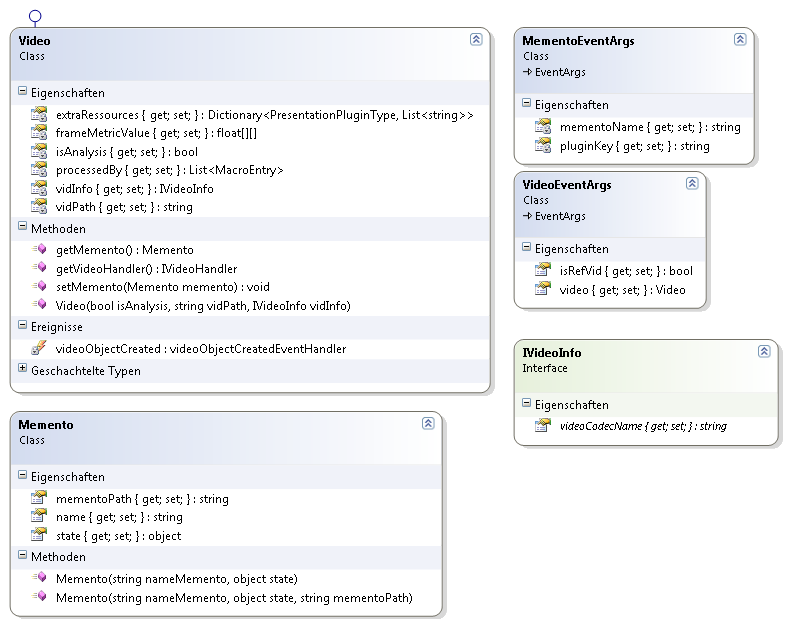
\includegraphics[width=\linewidth]{bilder/Klassendiagramm/publicModel.png}
\label{Private Model B}
\caption{Model B}
\end{figure}

\class{Video}{Klasse}
Im Video werden ein Pfad zu einer Videodatei, ein VideoInfo-Objekt sowie mögliche ">Extraressourcen"<, wie eine Datei zugehöriger Motionvektoren, gelegt. Falls es sich um ein Analysevideo handelt, werden zusätzlich entsprechende Analysedaten hier abgelegt. Ein Video kann außerdem auch einen VideoHandler zurück geben, mit dem auf die Video-Datei zugegriffen wird. Implementiert IMemorizable.


\class{VideoEventArgs}{Klasse}
Enthält ein Video und ein Boolean, der wahr ist, falls es sich um ein Referenzvideo handelt. Wird von Events als Argument benutzt.


\class{Memento}{Klasse}
Ein Memento speichert den Zustand eines Objektes. Es werden ein Name und gegebenenfalls auch ein Pfad zum Speichern auf die Festplatte bereitgestellt. Der Memento-Benutzer legt außerdem seine zu speichernden Daten ab.


\class{MementoEventArgs}{Klasse}
Enthält zwei Strings: Name eines Mementos und Referenz zu einem Plugin. Wird von Events als Argument benutzt.


\class{IMemorizable}{Interface}
Es wird ermöglicht, den Zustand einer Klasse als Memento zu speichern und vorherige Zustände zu laden.


\class{IVideoInfo}{Interface}
Falls ein Videoformat Voreinstellungen braucht bietet IVideoInfo die Möglichkeit diese abzulegen.

%\pagebreak
%\section{View}


\pagebreak
\section{ViewModel}

\subsection{Oqat Organisation}
\begin{figure}[H]
\noindent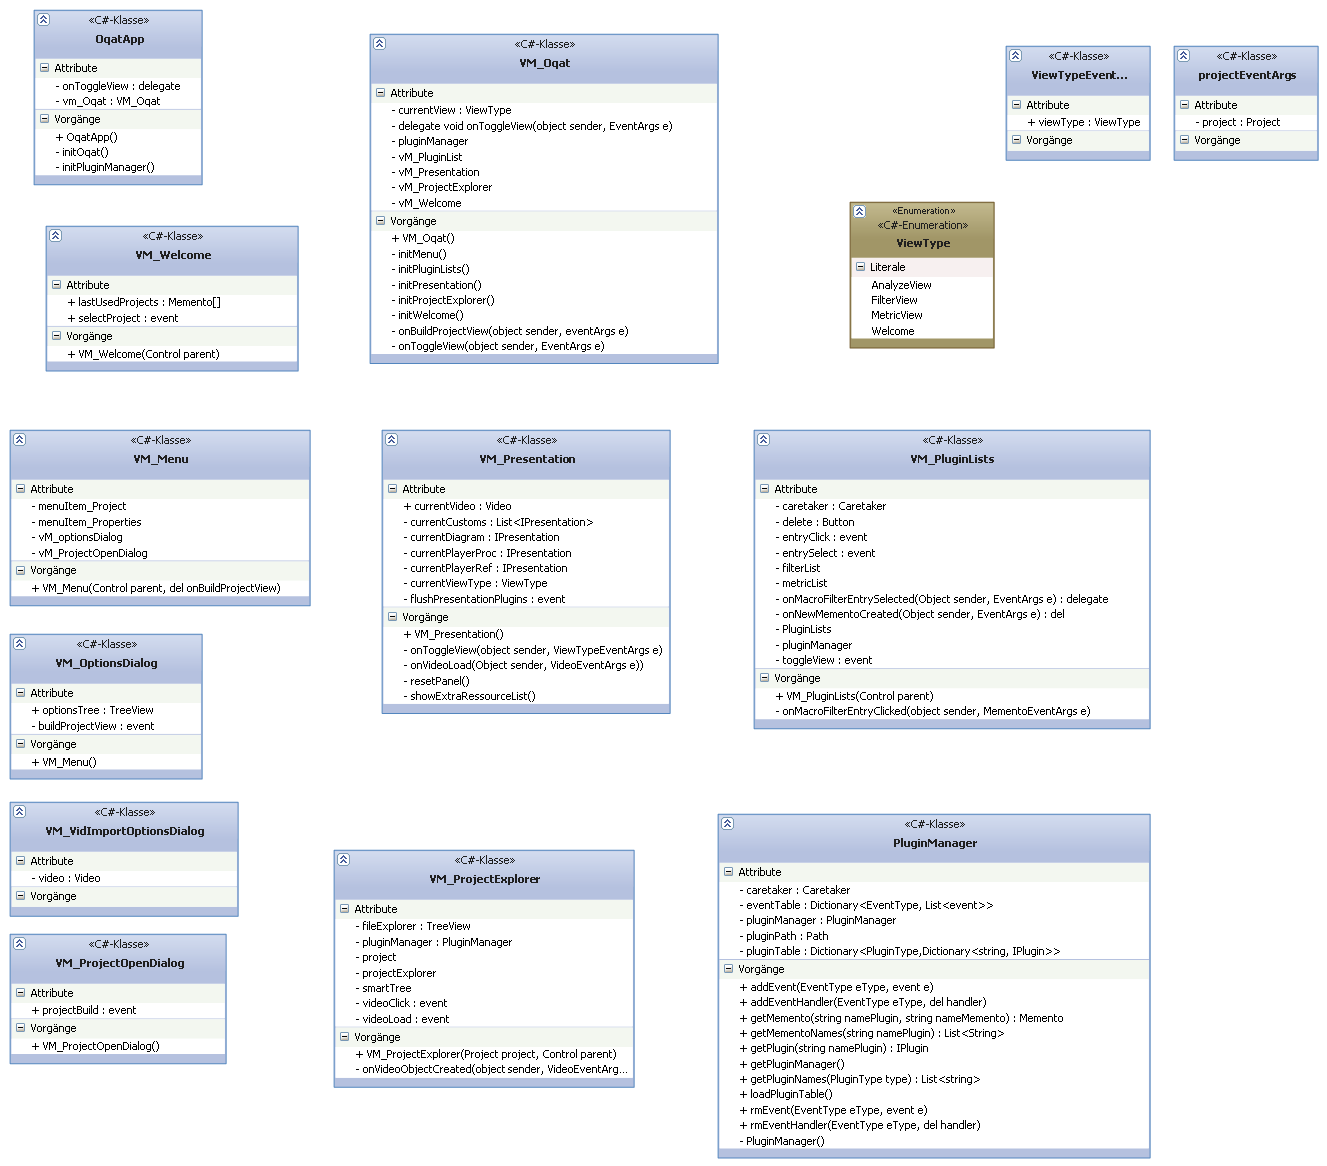
\includegraphics[width=\linewidth,height=\textheight,
keepaspectratio]{bilder/Klassendiagramm/VM.png}
\caption{Oqat Organisation}
\end{figure}

Alle sichtbaren VM (ViewModel) implementieren eine Methode onToggleView, die für den Ansichtswechsel zuständig ist und eventgesteuert funktioniert.

\class{OqatApp}{Klasse}
Die Klasse wird beim starten des Programms als erstes angesprochen und initialisiert die Anwendung und den Pluginmanager.


\class{VM Oqat}{Klasse}
Diese initialisiert die ViewModel Komponenten. Dazu gehören Willkommensbildschirm, das Projekt, Menü, Presentation und die Pluginlisten. Die Klasse stellt auch eine Delegate-Methode zum Ansichtswechsel bereit.


\class{VM ProjectExplorer}{Klasse}
Besteht aus einem SmartTree und einem Dateiexplorer, um diese in der GUI bereitzustellen. Er kann durch den Dateiexplorer Videos laden, diese werden im SmartTree angezeigt.


\class{PluginManager}{Klasse}
Der Pluginmanager ist die Schnittstelle zwischen \projektTitel und den Plugins. Er stellt Methoden zum Abrufen von Plugins und den zugehörigen Mementos. Außerdem werden Events mit deren Handlern bei ihm registriert.  Er ist als Singleton realisiert. Der Pluginmanager enthält einen Pfad zum Pluginordner sowie eine Tabelle, die den Plugintypen die zugehörigen Plugins zusammen mit deren Namen zuordnet.


\class{VM Pluginlists}{Klasse}
Die Pluginlist verwaltet die hinzugefügten Metriken und Filter, sowie die anderen Plugins. Er kann die Events entryClick und entrySelect abfangen. Bei entryClick wird ein Filter oder eine Metrik vom Container ausgewählt und die zugehörigen Einstellungen angezeigt. Bei entrySelect wird der ausgewählte Filter oder Metrik zu einer Makrowarteschlange hinzugefügt. VM Pluginlists stellt eine Delegatemethode bereit, die neu erstellte Mementos nach dem Abfangen des jeweiligen Events zu dem jeweiligen Plugincontainer hinzufügt.


\begin{figure}[H]
\noindent\includegraphics[width=\linewidth,height=\textheight,
keepaspectratio]{bilder/Klassendiagramm/VM2.png}
\caption{Oquat Organisation}
\end{figure}

\class{VM Menu}{Klasse}
Dieses ViewModel ist für die Verwaltung der Menüleiste und der Menüitems zuständig.


\class{VM Welcome}{Klasse}
Ist der Willkommensbildschirm, der beim Programmstart die zuletzt benutzten Projekte anzeigt.


\class{VM OptionsDialog}{Klasse}
Optionsfenster für allgemeine Einstellungen von \projektTitel.


\class{VM Presentation}{Klasse}
Der zentrale Visualisierungsbereich wird hiermit verwaltet. Dazu nutzt es die Presentationplugins um möglichst treffende Darstellungen zu erreichen.


\class{ViewTypeEventArgs}{Klasses}
Enthält ein Objekt vom Typ ViewType. Wird von Events als Argument benutzt.


\class{projectEventArgs}{Klasse}
Enthält ein Objekt vom Typ Projekt. Wird von Events als Argument benutzt.


\class{ViewType}{Enumeration}
In dieser Enum sind die verschiedenen Typen von Ansichten aufgelistet.

\class{VM ProjectOpenDialog}{Klasse}
Steuert das Fenster, das zum Öffnen eines Projektes verwendet wird.


\class{VM VidImportOptionsDialog}{Klasse}
Steuert das Fenster, das zum Importieren eines Videos verwendet wird.

\pagebreak
\subsection{Macro}
\begin{figure}[H]
\noindent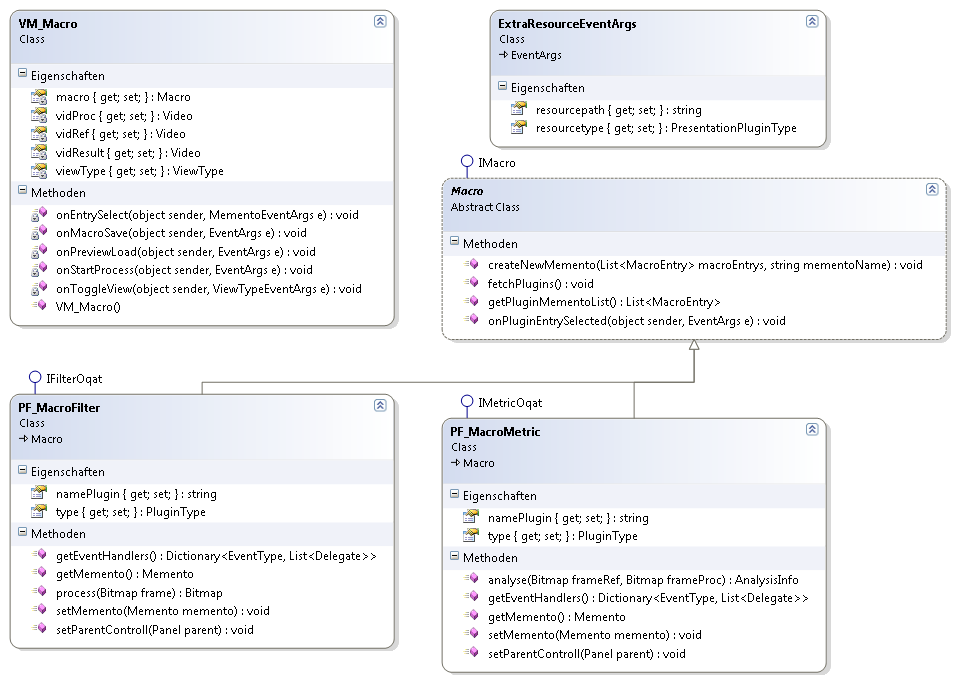
\includegraphics[width=\linewidth,height=\textheight,
keepaspectratio]{bilder/Klassendiagramm/Macro.png}
\caption{Macro}
\end{figure}


\class{VM Macro}{Klasse}
Legt fest, was bei einem Macro-bezogenen Event passiert. VM Macro kann Events vom Typ onEntrySelect, onMacroSave, onStartProcess und onToggleView abfangen. OnEntrySelect dient zur Auswahl von Filtern oder Metriken, die zum Macro zugefügt werden. OnMacroSave dient zum Speichern des Macrofilters. OnStartProcess startet den Macrofilter oder –analysevorgang. VM Macro enthält als Attribute ein Objekt vom Typ Macro, ein Objekt vom Typ Viewtype sowie Referenzen zu Videoobjekten.


\class{Macro}{Klasse}
Enthält eine Liste von MacroEntry-Objekten und implementiert IMacro.


\class{PF MacroMetric}{Klasse}
Erbt von Macro, implementiert IMacro und IMetricOqat. Diese Klasse bietet Methoden zur Analyse von Frames bzw. Videos an. Die Liste von MacroEntry-Objekten enthält in diesem Fall Referenzen zu Metriken, die durch diese Methoden angewandt werden können.


\class{PF MacroFilter}{Klasse}
Erbt von Macro, implementiert IFilterOqat. Die Liste von MacroEntry-Objekten enthält in diesem Fall Referenzen zu Filtern, die von einem MacroFilter durch die jeweiligen Methoden der Klasse PF MacroFilter auf Bilder bzw. ganze Videos angewandt werden können.


\class{ExtraResourcesEventArgs}{Klasse}
Enthält Pfad zu Extraressourcen sowie deren Typ. Wird von Events als Argument benutzt.

\pagebreak
\section{Plugins}
\subsection{Präsentation}
\begin{figure}[H]
\noindent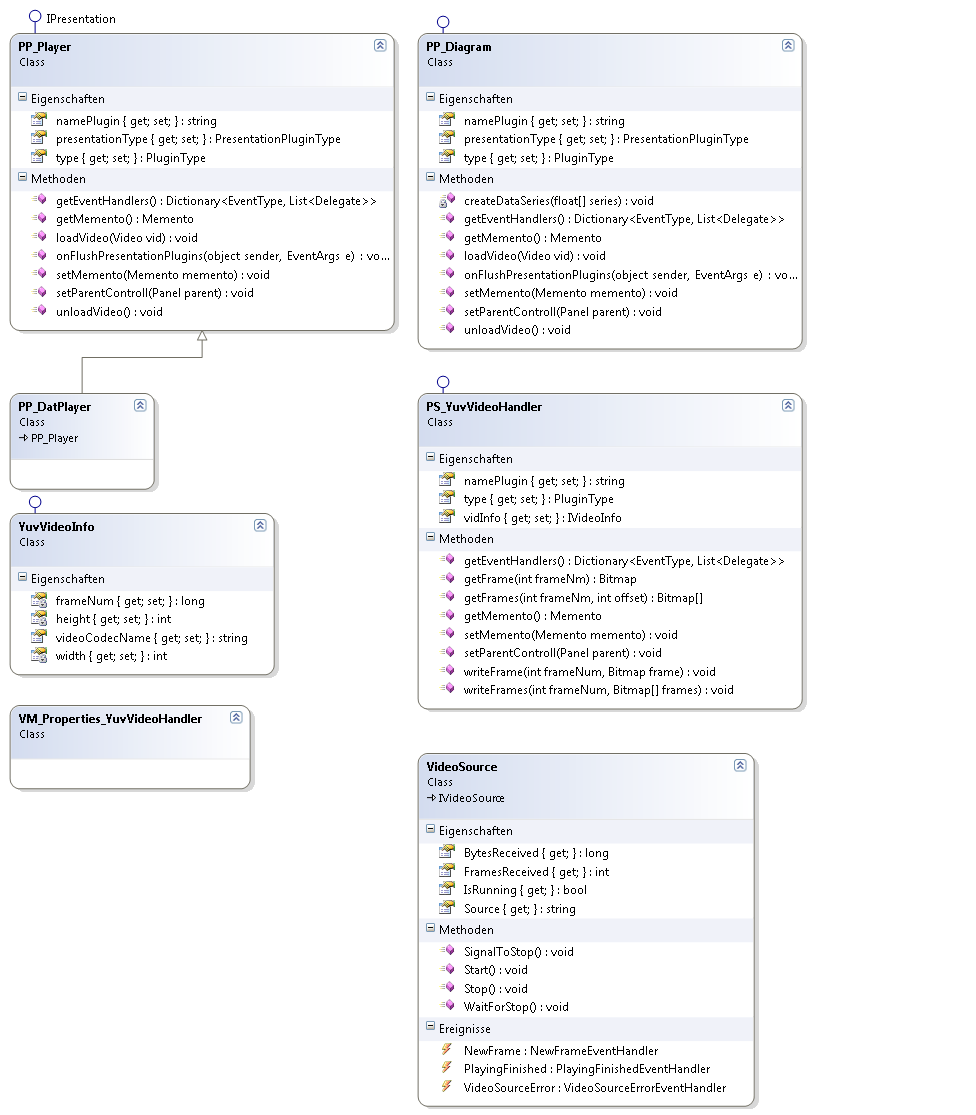
\includegraphics[width=\linewidth,height=\textheight,
keepaspectratio]{bilder/Klassendiagramm/Plugins1.png}
\caption{Presentation}
\end{figure}

\class{PP Player}{Klasse}
Stellt einen Container dem VideoSourcePlayer zur Verfügung. Lädt und entfernt die Videos, die von dem VideoSourcePlayer gezeigt werden sollen.


\class{PP Diagramm}{Klasse}
Stellt Oxyplot einen Container zum Zeichnen von Diagrammen zur Verfügung. Lädt und entfernt Videos, deren Attributen dann im Diagramm dargestellt werden können.


\class{VideoSource}{Klasse}
Die VideoSource dient als Adapter zwischen einem VideoHandler, der Videodateien liest und der vom AForge-VideoSourcePlayer benötigten VideoSource.
Implementiert IVideoSource von AForge. Implementiert Methoden zum Abspielen eines Videos.


\class{PP DatPlayer}{Klasse}
Erbt von PP Player und bietet dem VideoSourcePlayer die Möglichkeit, MotionVektoren (Dat-Dateien) als Overlays darstellen.


\class{PS YuvVideoHandler}{Klasse}
Erbt von IVideoHandler. Der YuvVideoHandler holt sich die Frames von einer YUV-Video-Datei bzw. schreibt sie wieder.


\class{YuvVideoInfo}{Klasse}
Enthält Informationen, die benötigt werden, um ein YUV-Video abzuspielen: Anzahl Bilder und Auflösung.


\class{VM Properties YuvVideoHandler}{Klasse}

\pagebreak
\subsection{Filter}
Die Plugins vom Typ Filter enthalten die jeweilige Arithmetik für den jeweiligen Filter. Spezielle Filter wie z.B. Blur werden als Memento abgelegt. Die dazugehörige VM kontrolliert das Einstellungsfenster der Mementos. Es wird IFilterOqat  implementiert.
\begin{figure}[H]
\noindent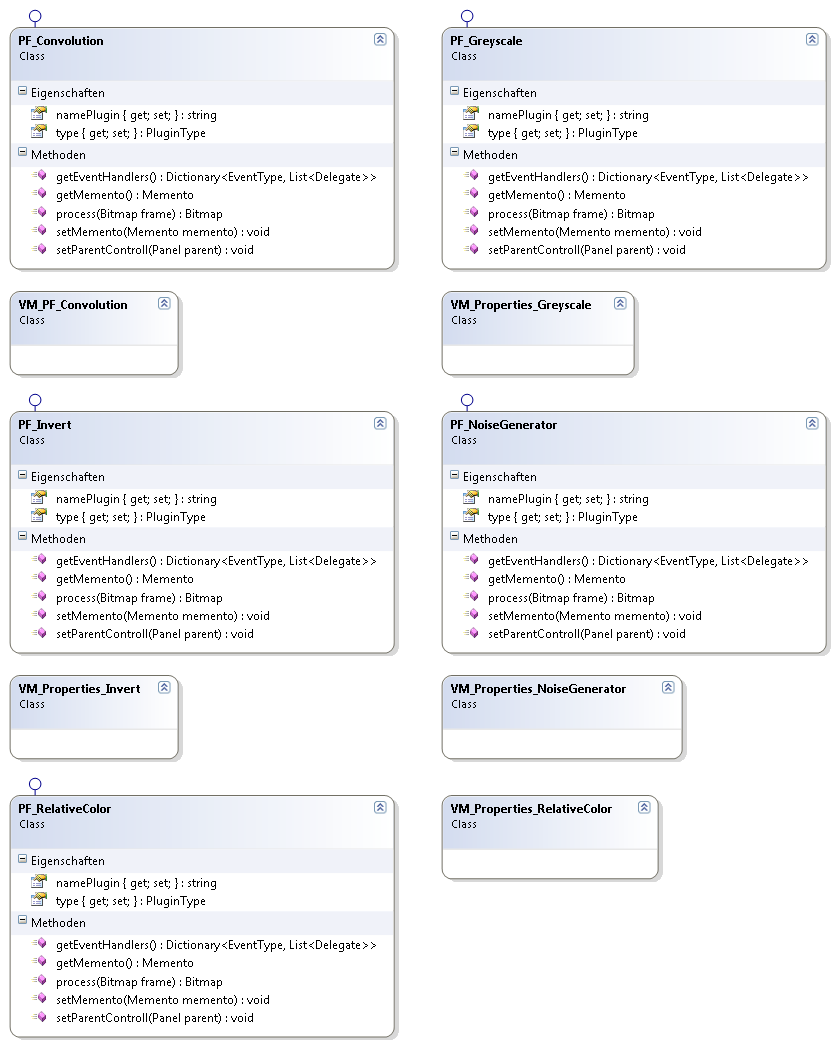
\includegraphics[width=\linewidth,height=\textheight,
keepaspectratio]{bilder/Klassendiagramm/Plugins3.png}
\caption{Filter}
\end{figure}


\pagebreak
\subsection{Metric}
Die Plugins vom Typ Metric enthalten die jeweilige Arithmetik für die jeweilige Metrik. Es wird IMetricOqat implementiert.
\begin{figure}[H]
\noindent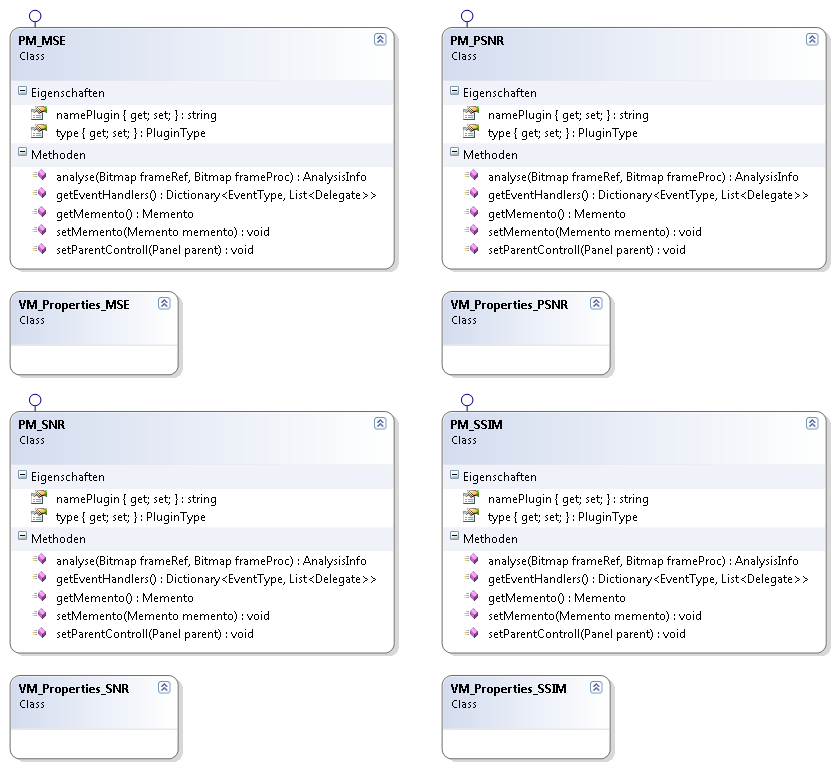
\includegraphics[width=\linewidth,height=\textheight,
keepaspectratio]{bilder/Klassendiagramm/Plugins2.png}
\caption{Metric}
\end{figure}

\pagebreak
\subsection{Oqat Public Ressources}
\begin{figure}[H]
\noindent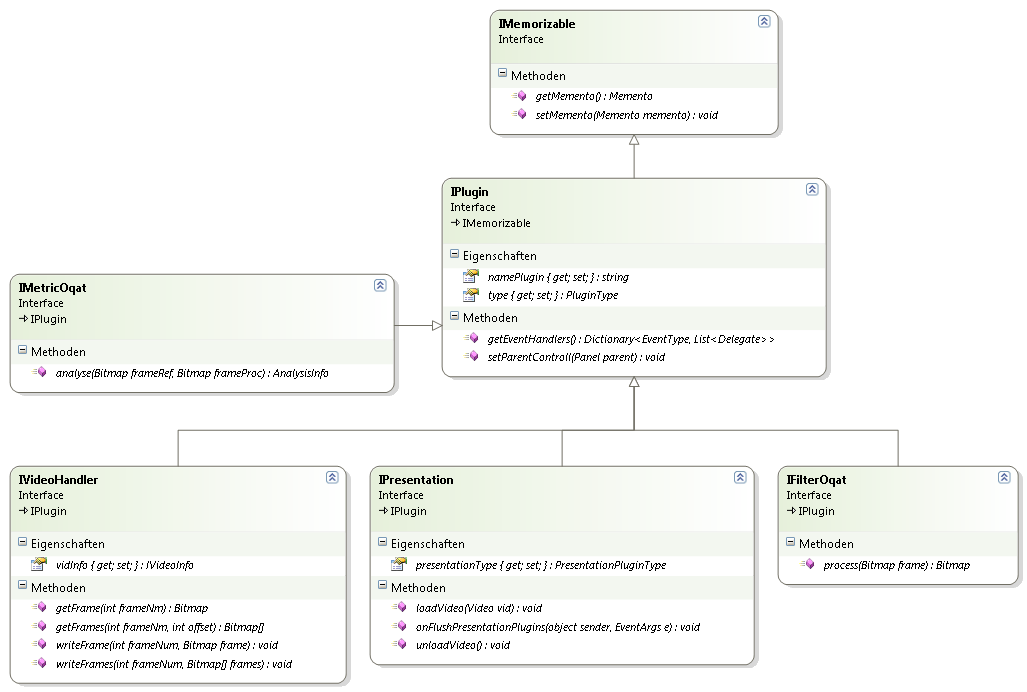
\includegraphics[width=\linewidth,height=\textheight,
keepaspectratio]{bilder/Klassendiagramm/PluginInterfaces.png}
\caption{Public Plugins}
\end{figure}

\class{IPlugin}{Interface}
Jede Klasse, die ein Plugin ist, muss dieses Interface implementieren. Namenattribut, Plugintypattribut und Methoden zur Verwaltung von Events (mittels Tabellen von EventTypen und den zugehörigen Delegatemethoden) werden dann von IPlugin geerbt. IPlugin implementiert IMemorizable.


\class{IPresentation}{Interface}
Implementiert das IPlugin Interface. Plugins vom Typ Presentation müssen dieses Interface implementieren. IPresentation bietet Methoden, um ein Video zu laden oder entfernen, und legt fest, was beim Entladen von Presentationplugins passiert.


\class{IMetricOqat}{Interface}
Implementiert das IPlugin Interface. Metriken müssen dieses Interface umsetzen. Es bietet eine Methode an, die für zwei Bitmap-Objekte ein IAnalysisInfo-Objekt zurückgibt.


\class{IFilterOqat}{Interface}
Implementiert das IPlugin Interface. Filterplugins müssen dieses Interface umsetzten. Es bietet eine Methode zur Bearbeitung von Bildern an, die ein Bitmap annimmt und wieder ein Bitmap zurückgibt.


\class{IVideoHandler}{Interface}
Implementiert das IPlugin Interface. Das Interface stellt Methoden zur Verfügung, die mit Frames in einem Video umgehen, indem man den Methoden eine Framenummer übergibt. Es bietet eine Methode an, mit der man sich einen bestimmten Frame holen kann, sowie eine Methode, an die man eine Framenummer und ein Offset übergibt und sich somit einen Array von Frames (Bitmaps) aus einem Video holt. Analog funktionieren die Methoden zum überschreiben von Frames.

\begin{figure}[H]
\noindent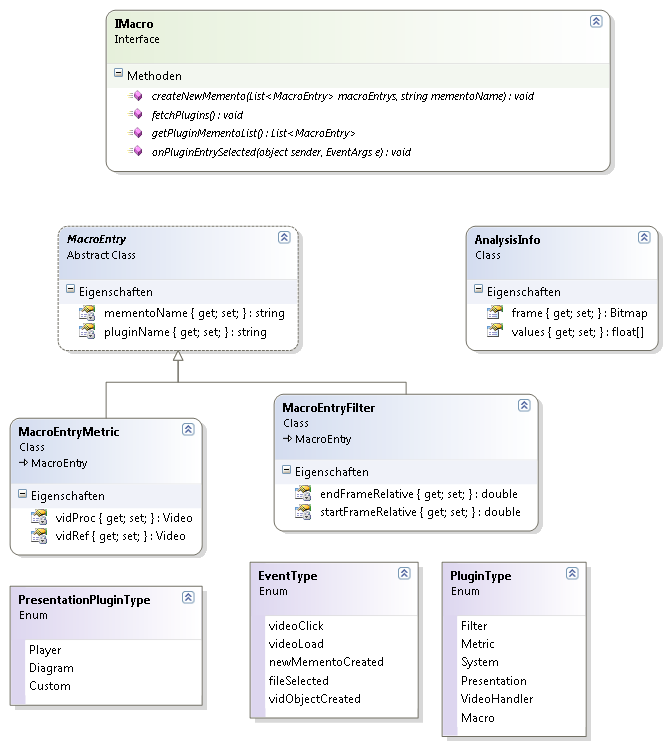
\includegraphics[width=\linewidth,height=\textheight,
keepaspectratio]{bilder/Klassendiagramm/PluginInterfaces2.png}
\caption{Public Plugins}
\end{figure}

\class{IMacro}{Interface}
Implementiert das IPlugin Interface. Ein Objekt vom Typ Macro muss dieses Interface implementieren. Es verwaltet eine Liste von Objekten vom Typ MacroEntry und bietet eine Methode, die aus so einer Liste und einem beliebigen Namen ein Memento-Objekt erstellen kann.


\class{MacroEntry}{Klasse}
Enthält zwei Stringattribute: eine Referenz zu einem Memento sowie eine Referenz zu einem Plugin.


\class{MacroEntryFilter}{Klasse}
Erbt von MacroEntry. Enthält zwei Double-Attribute: startFrameRelative und endFrameRelative. Ein MacroFilter kann auf Teile von Videos, die eine verschiedene Anzahl Frames besitzen, angewandt werden. Daher ist es sinnvoll, die Start- und Endframes für den Filtervorgang nur relativ zur gesamten Anzahl Frames anzugeben.


\class{MacroEntryMetric}{Klasse}
Enthält zwei Attribute vom Typ Video. Das sind die Videos, auf die eine Macrometric angewandt wird.

\class{AnalysisInfo}{Klasse}
Eine Metrik schreibt ihre Ergebnisse zuerst in ein AnalysisInfo-Objekt, damit dann später in das neue Video die Daten eingetragen werden können.


\class{PluginType}{Enumeration}
Der Enum enthält die Typen von Plugins.


\class{PresentationPluginType}{Enumeration}
Der Enum enthält die Typen von Presentationplugins.


\class{EventType}{Enumeration}
Der Enum enthält die Typen von Events.
